% !TeX root = ../main.tex

\chapter{Device evaluation and dispersion analysis}% from transmission spectroscopy

%\section{Methods}

In the example given in \autoref{sec:disp-comp},  a typical dispersive ring resonator has the $ D_2 $ value less than MHz, which means the frequency FSR, for example 100 GHz, is different from the next one with a MHz-level difference. It is difficult to achieve such precise measurement using traditional optical spectrum analyzer whose typical resolution is around pm, 100 MHz. The tunable laser scanning is developed to solve this problem, especially assisted by an external frequency comb \cite{Liu2016d}. 

Here, we exploit the method using laser step triggering to calibrate the real-time measured device transmission. Compared with the frequency comb or wave meter assisted spectroscopy, this method is much more convenient to deploy. By increasing the data acquisition sampling rate or altering with electric oscilloscope, the wavelength precision can be further improved.
Given the well-resonant spectrum, the dispersion information is further extracted from the transmission, in particular the resonant peaks. Such method is widely used to study the Kerr frequency comb. It is also efficient to study the frequency-entangled photon pair generation.

\section{Methods}

\subsection{Fiber launching}
Much of related works, concerning such as photonic crystals or whispering gallery mode resonators, use prism coupling or tapered fiber coupling for coupling tunability. 
%interact the external optical filed with cavity evanescent filed though, 
In the case of integrated ring resonators, the bus wavegudies are designed in the distance of several gaps, usually varying from under-coupling to over-coupling. 
Thus, the light confined in the bus waveguide can be directly coupled inwards or outwards using appropriate optical fibers. 
In previous works \cite{Sunada2018}, both grating coupling and edge coupling were adopted. However, considering the broadband frequency conversion motivation, the edge coupling is preferred for a comparatively broader 3-dB bandwidth. 
 
Using two five-axis fiber alignment stages (Newport M-562F-XYZ \& M-562F-XYZ-LH), the device ports are aligned with the lensed fiber on both sides. The spot size of lensed fibers is 2 \si{\um}, which is not optimized to the size mentioned in \autoref{sec:chip-dicing}.
In the case of ligentec samples,  the best facet-to-facet coupling efficiency is around 6 dB. 
Comparatively, a more typical facet-to-facet loss without mode convertors can be 8-9 dB.

%LS-CVD samples

It is worth mentioning that a chip arrier (SURUGA SEIKI F126) equipped with a thermoelectric cooler (TEC) is specialized for the \textit{xz}-axis device stage, which is essential for long-time thermal stability. 
With connected to an external temperature controller, the temperature precision of device under test can be .1 \si{\celsius}.
To prevent moisture condensation, the TEC is set a little bit higher than room temperature, 30 \si{\celsius} in our case. 

\subsection{Spectrum sweeping}

\begin{figure}
	\centering
	\includesvg[width=.9\textwidth]{trans_setup}
%	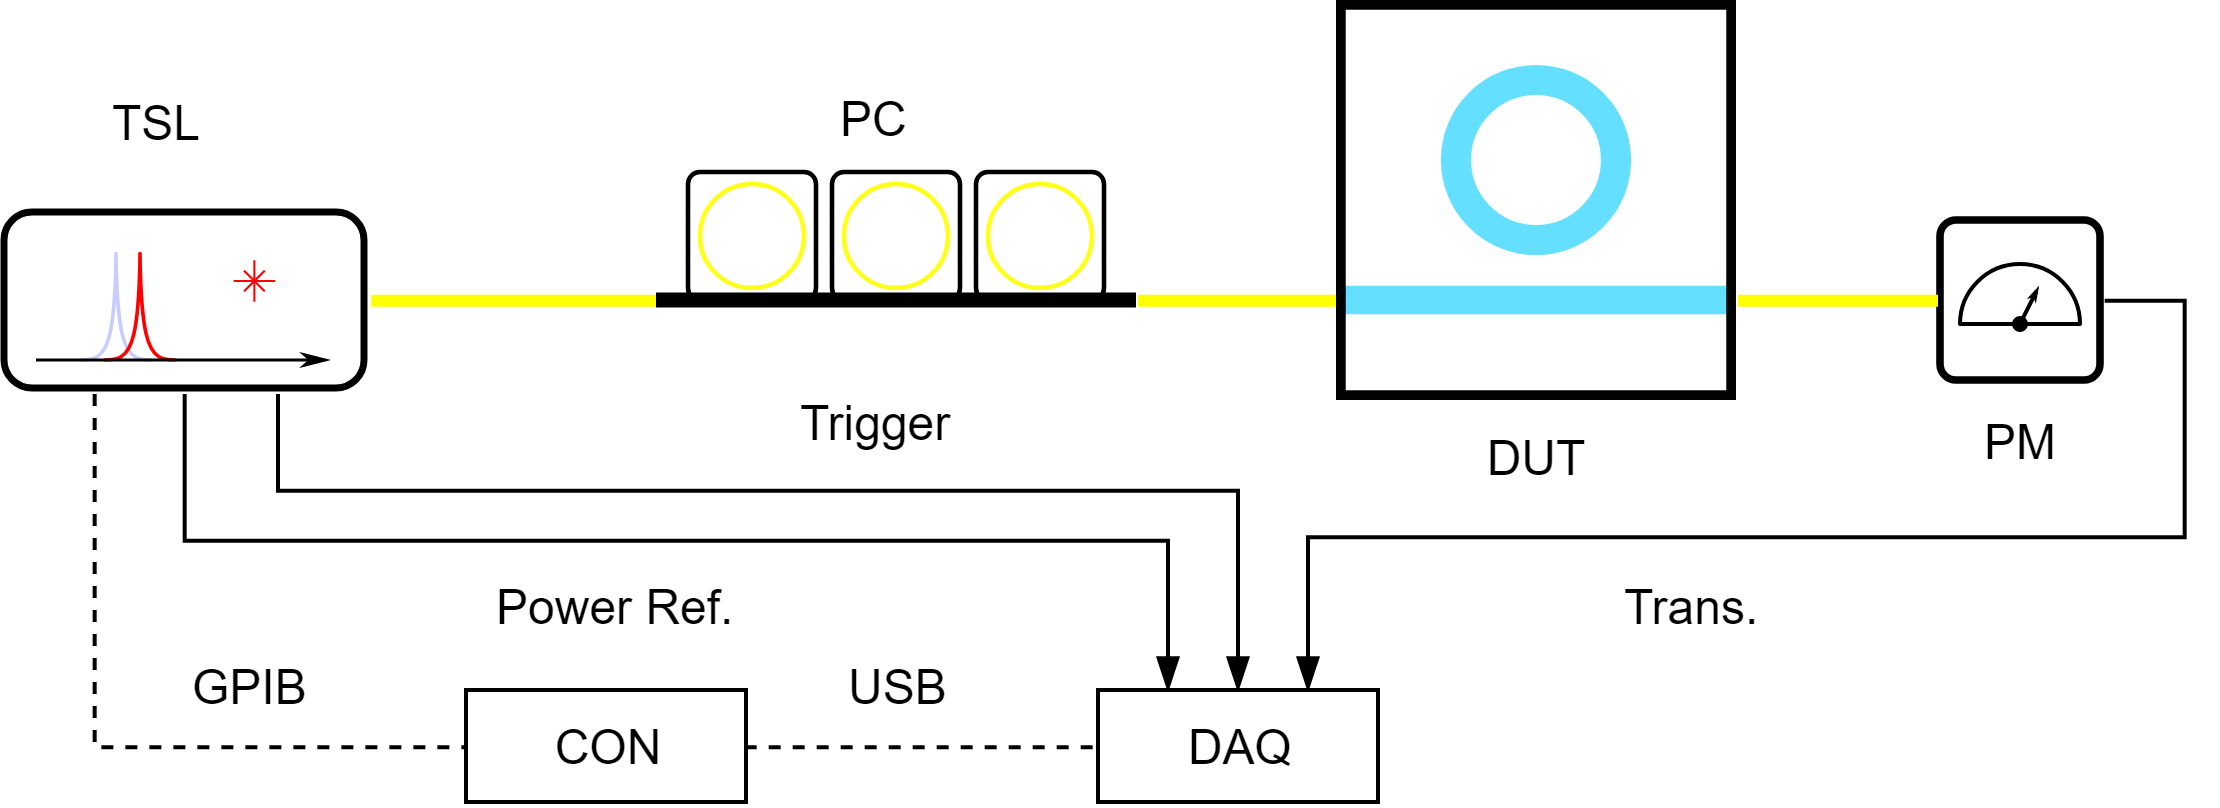
\includegraphics[width=.9\textwidth]{imgs/png/trans_setup}
	\mycaption{Setup of transmission measurement system}{TSL, tunable semiconductor laser. PC, optical fiber polarization controller. DUT, device under test. PM, power meter. DAQ, data acquisition.}
	\label{fig:transsetup}
\end{figure}

The schematic diagram of the device spectrum measurement is shown in \autoref{fig:transsetup}. Before the spectrum scanning, the output port is coupled to the infrared InGaAs camera in free space using a 20$\times$ objective lens. By carefully rotating the palette of polarization controller on the input side, the device can be launched in either TE or TM mode. Next, the TSL (SANTEC TSL-710) is set to continuously sweep from 1480 nm - 1640 nm, covering the telecom S C and L bands. The internal power reference signal and the step trigger are also generated simultaneously. Compared with photon diodes, the power meter (Newport 2963-R) in our setup is critical to realize the scanning at various power ranges.  Finally, the signals from power monitor, step trigger and device transmission are all synchronized with the data acquisition module, and then analyzed by the computer.

Given the transmission spectra, the negative peaks are located with peak-finding algorithm, yielding not only the peak location, but also the width and prominence, which are used to calculate the free spectral range and \textit{Q}-factor.

% \section{Results}
\subsection{Dispersion analysis}
Previous work \cite{Sunada2018} gave two methods analyzing the device dispersion. One is to perform Fourier transform of the reflected spectra on the input port, which is equivalent to the interference in a $2L$-long etalon. Another method is similar but using the resonance in the cavity instead. 

Despite the fabrication tolerance, considering the bent segment, the chromatic dispersion in the ring resonator is not identical to the one in the straight waveguides. Hence, in our research, to the extract the dispersion information accurately, the ring resonacen method is employed. 

Following the integrated dispersion definition, the resonant wavelength $\lambda_m$ is first converted to resonant frequency $\omega_m$. Before the polynomial fitting to the frequencies, the linear fitting is performed to evaluate first-order mode dispersion parameters and then used to calculate the integrated dispersion using the formula $ \dint(\mu) = \omega_0 - D_1 \mu$. The central frequency is $\omega_0$ set as the center of scanning range. The relative mode numbers are constructed as a integer neighbourhood of zero. A final step is perform the cubic or quadratic polynomial fitting. For the wide range scanning, a quartic curvature is more efficient, but in our case, the cubic polynomial is sufficient to extract the dispersion parameters at the second order in a 160 nm span.

\section{Thermal stability}

\begin{figure}
	\centering
	\includesvg[width=1\textwidth]{thermal}
	%	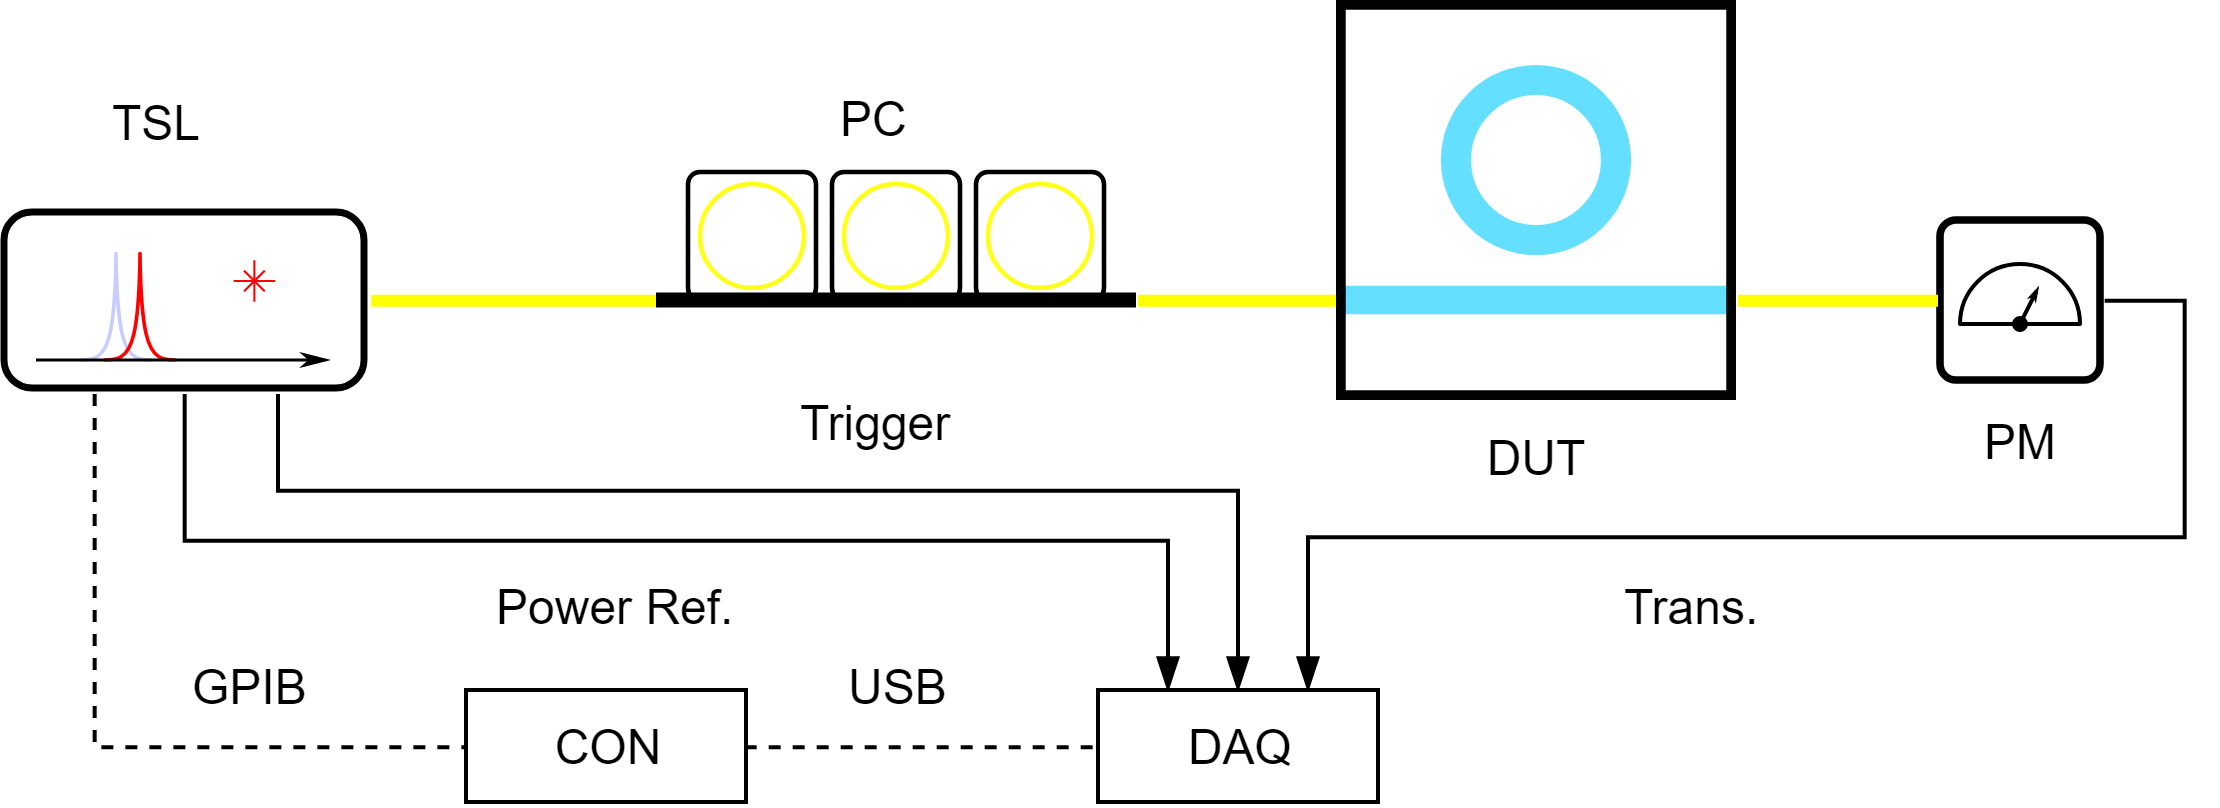
\includegraphics[width=.9\textwidth]{imgs/png/trans_setup}
	\mycaption{Transmission}{}
	\label{fig:thermal}
\end{figure}

%\begin{figure}
%	\centering
%	\includesvg[width=.9\textwidth]{dwldT}
%	%	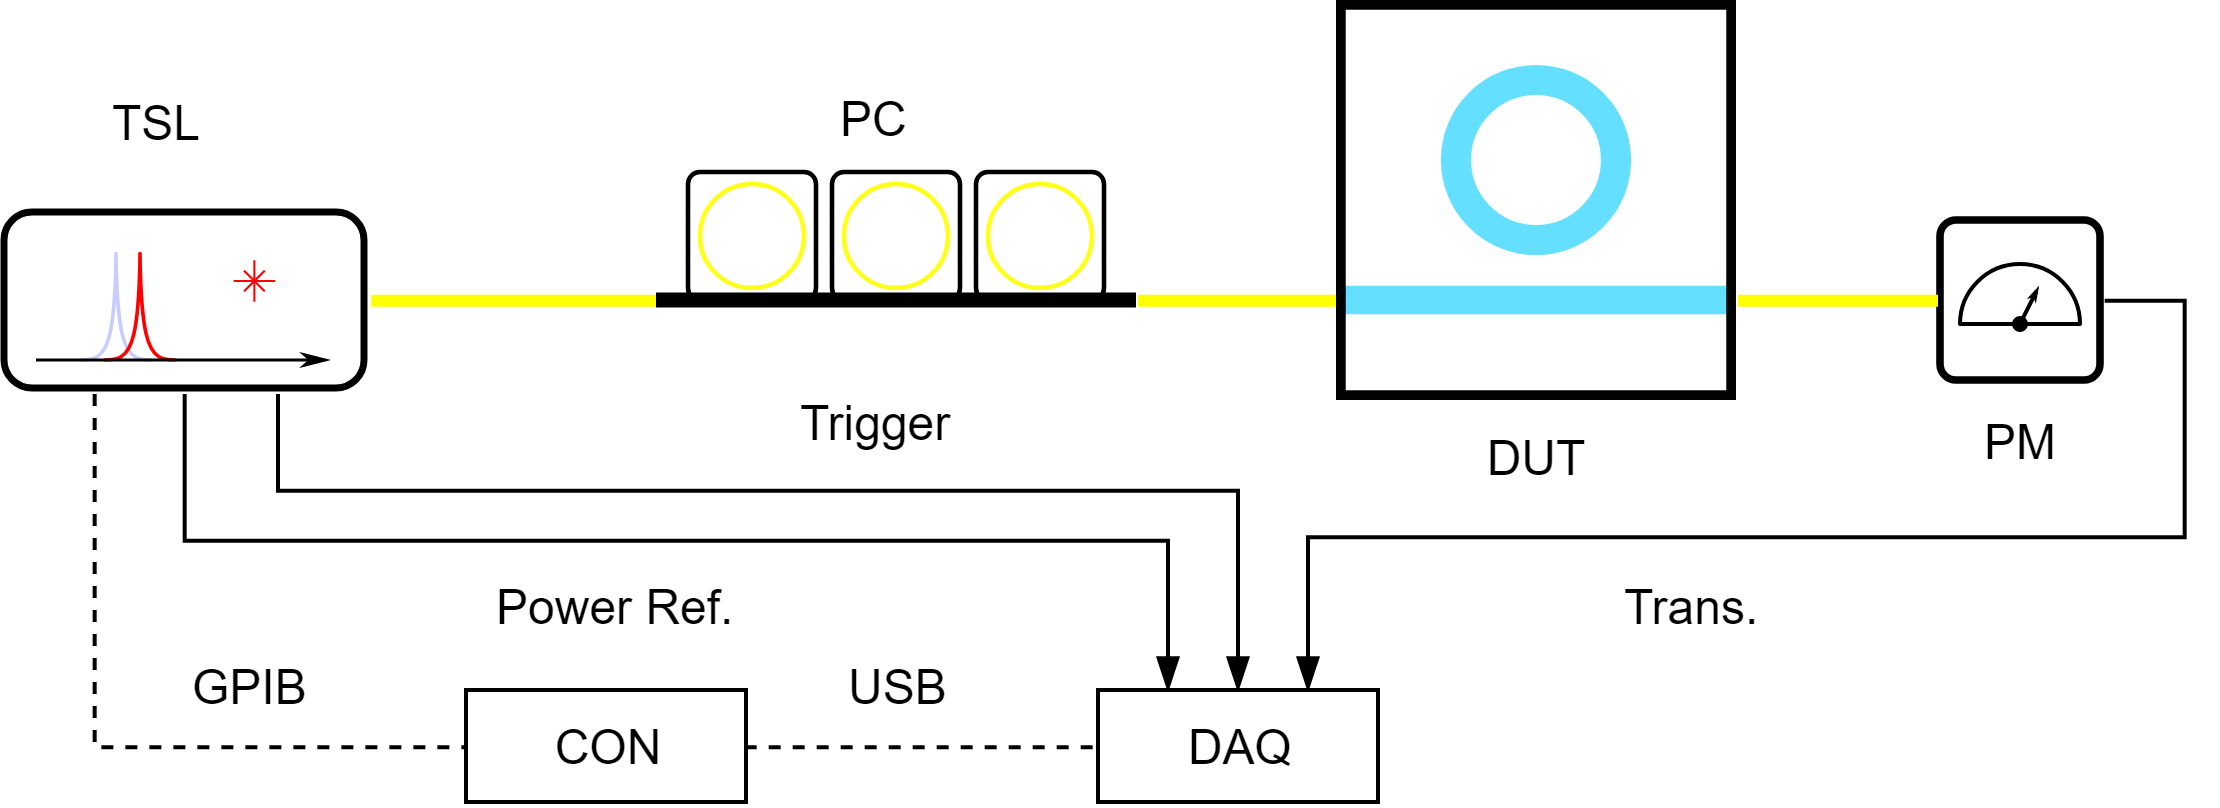
\includegraphics[width=.9\textwidth]{imgs/png/trans_setup}
%	\mycaption{}{}
%	\label{fig:wl-T}
%\end{figure}

Although silicon nitride is reported as high thermal conductivity material, the surrounding silicon dioxide is comparatively worse thermal-conductive. Despite the room temperature fluctuation, the nonlinear phenomena usually requires high pump power intracavity, which heats the device significantly, the index change variation leads to resonance shift. Thus, the thermal sensitivity is a critical factor of nonlinear ring resonators.

For example, with the TEC set into different temperatures, the spectrum of a LP-CVD sample is then measured. Shown in \autoref{fig:thermal}a, temperature increasing leads to a obvious red-shift of the resonant peak. The wavelength range around 1630 nm is chosen for better transmission and well resonance in this device. From \autoref{fig:thermal}b, the estimated thermal dependence of resonant wavelength $\dv*{\lambda}{T}$ is 23 \si{\nm/\celsius}. In this case, if the \textit{Q}-factor of ring resonator is up to \num{10d5}, even room temperature variation can results in resonance totally mismatching at pumping wavelength.

\section{Device transmission}

\subsection{Substractive fabricated samples}

To compare the material difference among the films deposited in three CVD methods, identical layout is used to fabricate the ring resonators using all the same recipes. %Controlling thickness 
Since the thickness control during the film deposition and ICP etching is tough, all the device are label with the waveguide height measured by step profiler before TEOS top cladding. However, the fabrication of stoichiometric silicon nitride using PE-CVD method is not successful, a sample deposited using same machine but with a silicon-rich recipe is reported instead. 

The device transmission spectrum is first measured, shown in \autoref{fig:trans_cf}. It can be seen that there is strong optical absorption from 1520 nm to 1540 nm in each device. Compared with the FTIR result shown in \autoref{fig:ftir}, in particular the case of LP-CVD sample where is almost no Si-H or N-H bonds found, the absorption at optical telecom band not only originates from the residual hydrogen but also may results in top-cladding or bottom buried TEOS layer.
In addition, LP-CVD sample shows absorption at some certain wavelength, leading to the error values of peaking finding. Such kind of broken spectra can be probably explained by the fabrition toleration, such like the gap is not fully etched or the ring resonator is contaminated with a certain particles. All these fabrication imperfection plays the role of sacttering and also decreases the quality factors.

Furthermore, from the extracted resonant peaks, the \textit{Q}-factors and frequency FSRs are summarized in \autoref{fig:QF_cf}. The radius of each ring resonator are designed as 200 \si{\um}, corresponding to the FSR of 119.3 GHz. This agrees with the extracted FSRs of LP-CVD and LS-CVD samples. In the case of silicon-rich PE-CVD sample, the measured FSR of ring resonators near 1550 nm is around 94.3 GHz, indicating the refracting index of silicon-rich silicon nitride film is 0.34 higher.

% \si{\percent} 
In the term of \textit{Q}-factors, counted in \autoref{fig:Qhist}, the LS-CVD samples have the highest quality values at the mean of \num{3d4} while the one of silicon-rich PE-CVD samples is near to \num{1e4}. The distribution of LP-CVD sample are similar to LS-CVD ones, but influenced by the broken resonance spectrum.

\begin{figure}
	\centering
	\includesvg[width=.8\textwidth]{trans_cf}
	\mycaption{Trans Comparison}{}
	\label{fig:trans_cf}
\end{figure}

\begin{figure}
	\centering
	\includesvg[width=.8\textwidth]{FSR_Q_new}
	\mycaption{FSR cf}{}
	\label{fig:QF_cf}
\end{figure}

\begin{figure}
	\centering
	\includesvg[width=.8\textwidth]{QHist_cf}
	\mycaption{Q histogram}{}
	\label{fig:Qhist}
\end{figure}

